\section{Domain Model}
The domain model provides clarity and direction for a software system, even on a small scale such as in a library. In this section the design choices of the data model will be discussed.

\subsection{Data Model Overview}
In order to capture the data model in an object-oriented programming language, a UML diagram was maintained as the implementation went along in order to keep track of relationships between the classes. 
% As a general rule of thumb, all the fields were made public including those required by the constructors, and the methods of the classes were all \textit{getters}, i.e. \\

\subsubsection*{GeoPosition}
A \textit{GeoPosition} is defined by a geographical \textit{latitude} and \textit{longitude} and represents a 2D position on the Earth's surface.

\subsubsection*{Location Sample}
A \textit{Single Location Data Point} is a time-stamped \textit{Location}. By having a time-stamp, a collection of Location Samples may be ordered and grouped by the time of day. In essence, the class is a Data Transfer Object (DTO) \footnote{\url{https://martinfowler.com/eaaCatalog/dataTransferObject.html}} which is used to transfer GPS data from an arbitrary Location plugin to the \textit{Mobility Features Package}.

\subsubsection*{Hour Matrix}
An \textit{Hour Matrix} is a matrix with 24 rows and columns equal to the number of places of some period. The \textit{Hour Matrix} class is used to calculate the \textit{Routine Index} feature, as well as to identify the \textit{Home Cluster}, which is the place most visited during 00:00 and 06:00. An Hour Matrix is constructed from a list of \textit{Stops} which all have the same date.

\subsubsection*{Stop}
A \textit{Stop} is constructed from a centroid of a data point cluster (i.e. a Location) in addition to an arrival- and a departure timestamp, and a place ID indicating which place it belongs to.

\subsubsection*{Place}
A \textit{Place} is constructed from a place ID, as well as a collection of \textit{Stops} belonging to that \textit{Place}. 

\subsubsection*{Move}
A \textit{Move} is constructed from a pair of \textit{Stops} as well as the set of \textit{LocationSamples} which were sampled in between the two \textit{Stops} which is the path the user took between the two \textit{Stops}.

\subsubsection*{Mobility Context}
A \textit{Mobility Context} is a collection of features which are derived from a set of intermediate features, where the \textit{Stops} and \textit{Moves} are from a specific date. The \textit{Places} is derived from multiple dates for reasons which will be explained in the implementation details. In addition, a set of \textit{Mobility Contexts} from previous dates can be provided as an optional parameter. A Mobility Context contains the mobility features, although the \textit{Routine Index} is only available if an array of the set of \textit{Mobility Contexts} was provided as a parameter, which is due to the feature depending on the data from previous days in order to compare them.

\subsubsection*{GeoSpatial (Interface)}
This interface will impose a getter-method for the GeoPosition of the class which implements it. This allows the Haversine distance to be calculated between objects of different types.

\subsubsection*{Serializable (Interface)}
This interface will impose a serialization and de-serialization method for converting between a language object and a JSON object. The interface will allow the MobilitySerializer component as previosly discussed to more easily implement serialization in a generic manner which is disucssed in Chapter \ref{chapter:05}.

\subsection{UML Diagram and Discussion}

\begin{figure}[h]
    \centering
    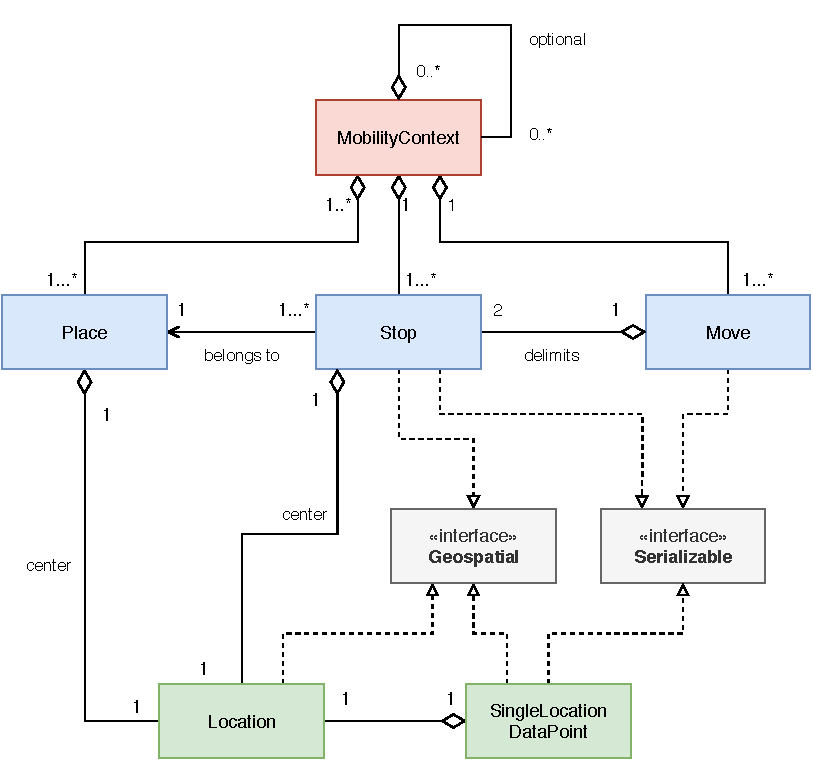
\includegraphics[width=0.7\textwidth]{images/diagrams/uml.pdf}
    \caption{UML diagram for the classes used in the \textit{Mobility Features Package}}
    \label{fig:my_label}
\end{figure}

The data model could be modified such that a Place contained a list of \textit{Stops} made at that place, rather than using both \textit{Places} and \textit{Stops} for instantiation of \textit{Mobility Context}. This would mean grouping the \textit{Stops} by Place rather than date, and would require filtering to take place every time a \textit{Mobility Context} object is created, to remove all Stops, not on that specific date. In a real-world scenario the application developer will likely have the Location Samples for the current day available, and from those the \textit{Stops} today can be generated which means no filtering is required. Grouping \textit{Stops} into places would however lead to a nicer data model, but a design choice was made in favor of less computation. 


